\chapter{Technical Foundations}

\section{Introduction}
For the purpose of this project, an extensive investigative study into Retrieval-augmented Generation process has been conducted. This chapter explains RAG in more detail, explores its paradigms, outlines its components and provides the rationale behind the selection of certain choices.

\section{RAG Overview}
Retrieval-augmented Generation, or RAG for short, is an information retrieval pipeline consisting of mainly two consecutive processes: Retrieval and Generation.
\begin{itemize}
    \item The purpose of the first phase (retrieval) is to fetch, from a knowledge base containing a large number of documents, the passages that are most relevant to a given query. It gets initiated when a user submits a question to the system, and depending on the indexing method of the knowledge, calculates and determines a collection of short text paragraphs containing relevant data. This information constitutes the "context" in RAG glossary, and gets then passed to the next phase along with the input question.
    \item The second phase focuses on generating a suitable response for a given query. It achieves this by first structuring an instruction, composed of the question and context from the previous phase, in a format interpretable by a generative AI model. The model then analyses the instruction (or prompt) and based on its architecture, attempts to generate a suitable response.
\end{itemize}
The RAG technique represents a method for customizing the interaction with a generative AI model, and enables to control the referenced information in the generation process. In the next section, we explore some approaches to designing the overall pipeline and how to tailor its processes for more accurate results and better performance.

\section{RAG Paradigms}
The RAG process has significantly improved on the limitations of generative AI models by augmenting their knowledge while eliminating the need to re-train them. Even so, a simple RAG pipeline can still exhibit various flaws, such as retrieval-echoing generation, which means responding with the contents of the retrieved documents rather than adding more insights through the Generative AI models' capabilities. Moreover, this baseline RAG can still introduce hallucinations by confining the generative process to the retrieved documents, which may not be pertinent to the query in every occasion, such as in case where relevant information are not present or cannot be retrieved from the knowledge base. In this respect, as more research and engineering is continually being conducted, advanced spinoffs of RAG has emerged to reduce the mis-reckoning and limitations of simplistic RAG.
\begin{figure}[H]
    \centering
    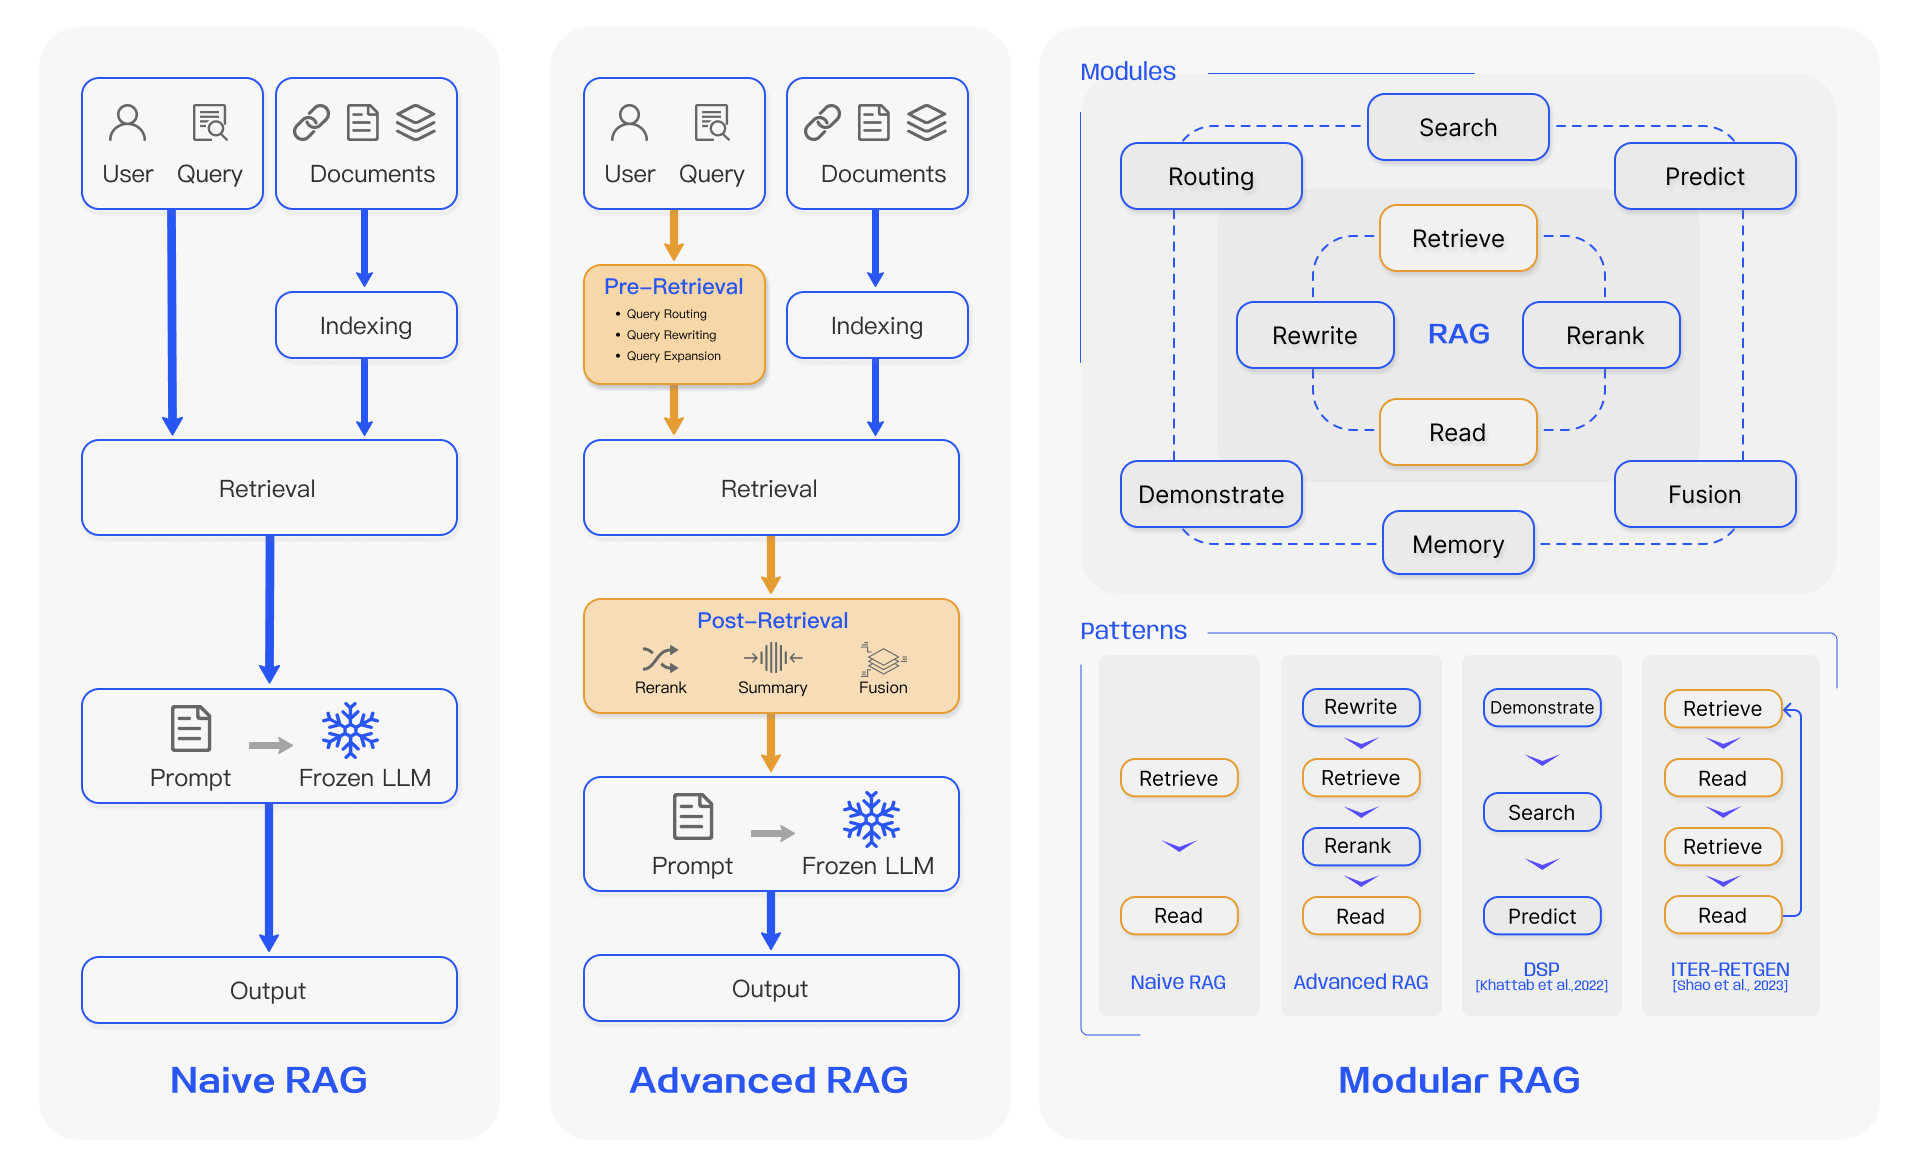
\includegraphics[width=\linewidth]{./figures/RAG_FrameCompre_eng.png}
    \caption{Comparison between the three paradigms of RAG: Naive, Advanced and Modular RAG \cite{ragforllmsasurvey}}
    \begin{flushleft}
        \small Naive RAG (LEFT)  mainly consists of three parts: indexing, retrieval and generation. Advanced RAG (MIDDLE) proposes multiple optimization strategies around pre-retrieval and post-retrieval, with a process similar to the Naive RAG, still following a chain-like structure. Modular RAG (RIGHT) is not limited to sequential retrieval and generation; it includes methods such as iterative and adaptive retrieval.
    \end{flushleft}
\end{figure}
In the light of this, we focus on the advanced RAG pipeline structure, which addresses many of the shortcomings of a naive RAG chain without introducing too much complexity to the overall pipeline, which results in very long question-to-generation delays and expensive API calls.
This paradigm involves knowledge base augmentation by routing the input query to other processes and external knowledge sources such as web content searching and generative research conducting, translating text across languages, context summarization and re-ranking, and LLM instructing through prompt engineering in addition to the evaluation and re-ranking of the generation phase' results. This is achieved through the introduction of two additional steps or processes into the overall pipeline: pre-retrieval and post-retrieval. The pre-retrieval phase focuses on selecting knowledge sources from which the context can be retrieved (query routing), translating the question if needed (query rewriting) and connecting it to external knowledge sources e.g. search engines and AI research generator (query expansion). The post-retrieval phase focuses on constructing the best prompt by interpolating and prioritizing more relevant context into it while eliminating unrelated parts. This phase also addresses content overload by filtering recurrent and repetitive information, compressing or summarizing context, and finally, as a post-generation step, re-ranking generated answers (in our case of multiple LLMs). These extra steps would result in better user experience in case knowledge base augmentation is required just-in-time of answer-generation or a re-ranking/adjustment of either retrieval or generation phase output is required.\bigskip\newline
Having highlighted the mains steps of the RAG pipeline, it is now worth examining the different components that needs to be integrated in the system and the interaction between them, which will be discussed in the next section.

\section{System Architecture}
The different processes and subprocesses which a RAG pipeline involves require a number of discrete components that, with their synergistic functioning, constitute the framework behind the operation of this chain.\newline The overall pipeline structure is illustrated in the following figure, which showcases the interaction between these individual components.\newline
\begin{figure}[H]
    \centering
    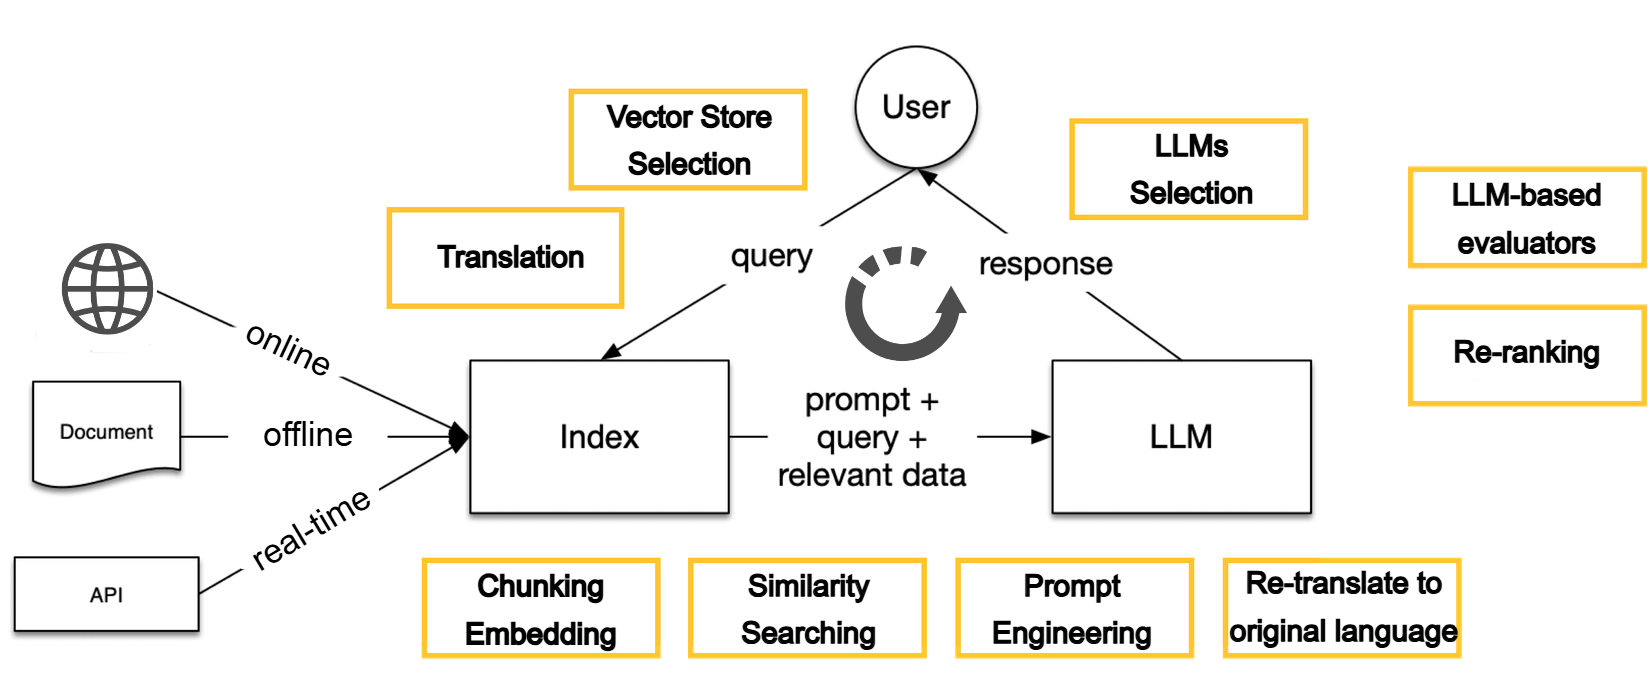
\includegraphics[width=\linewidth]{./figures/rag_components.png}
    \caption{The composition of the system's RAG pipeline}
\end{figure}
This figure demonstrates the overall processes that are executed in the system, incorporating the following concepts:
\begin{itemize}
    \item Vector Store (Index): Is a type of a database suitable for storing large volumes of documents that needs to be queried efficiently. This repository represents the Entreprise Knowledge Base.
    \item Data ingestion: Refers to the sources from which the knowledge base can be augmented.
    \item Embeddings Model: is an algorithm that transforms text (or other data) into numerical representations called embeddings, capturing semantic and syntactic information, which enables the vector store to find the most relevant information based on a query.
    \item Generative AI model (LLM): This is a type of a ML model that can analyze textual input and generate output accordingly.
    \item Prompt: A set of instructions and other information that elicits a certain output or behavior from the generative model.
    \item Other AI models: Used for translating text between languages, and re-ranking and compressing the retrieved context.
\end{itemize}
The following subsections are dedicated to the exploration of these elements and selecting concrete tools from these concepts.
\subsection{Vector Stores}
'Vector Store' refers to a type of database responsible for the storage and indexation of documents and other unstructured data in a numerical representation suitable for retrieving relevant parts from large volumes of data through similarity searching algorithms.
\begin{quote}
    "Traditional databases are made up of structured tables containing symbolic information. For example, an image collection would be represented as a table with one row per indexed photo. Each row contains information such as an image identifier and descriptive text. Rows can be linked to entries from other tables as well, such as an image with people in it being linked to a table of names.

    AI tools, like text embedding (word2vec) or convolutional neural network (CNN) descriptors trained with deep learning, generate high-dimensional vectors. These representations are much more powerful and flexible than a fixed symbolic representation, as we’ll explain in this post. Yet traditional databases that can be queried with SQL are not adapted to these new representations. First, the huge inflow of new multimedia items creates billions of vectors. Second, and more importantly, finding similar entries means finding similar high-dimensional vectors, which is inefficient if not impossible with standard query languages."  \cite{faissess}
\end{quote}
This specific type of database provides many functionalities and processes pertinent to the functioning of a RAG pipeline, which are explored in the following subsections.
\subsection{Chunking}
First of all, when indexing large documents into the knowledge base, one should consider the size of this contiguous information and the context window limitation of LLMs, as each model has some limit on the amount of information it can receive as context. In these conditions, a chunking of documents should be implemented before the embedding and storing phases. This technique allows to divide documents into smaller passages, while marking these with metadata (document id, order etc...) which would allow the vector store to structure and store these chunks as if they were a monolithic record.\newline
The following figure demonstrates the initial steps when a new data source is being recorded into the knowledge base.
\begin{figure}[H]
    \centering
    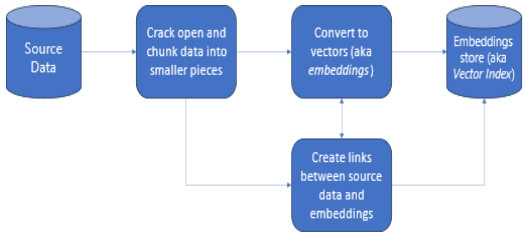
\includegraphics[width=.7\linewidth]{./figures/chunking-embedding-diagram.png}
    \caption{Embedding Document Chunks Diagram. (Microsoft, 2023)}
    \begin{flushleft}
        When loading new information into the vector store, a segmentation of the content needs to occur before transforming it into numerical representation. The chunking phase achieves this by splitting the document into a fixed length chunks, creating links between them and then passes to next phase of vectorization or embeddings generation, which is discusses below.
    \end{flushleft}
\end{figure}
\subsection{Vectorization}
Embedding vectors, as in vector store, are arrays of floating-point numbers produced by embeddings models. The output of these models captures the semantics of the vectorized text. This representation is suitable for RAG applications because these embeddings are computed in a way that semantically similar information have similar values, which allows for efficient indexation and similarity search algorithms' implementation.
\begin{figure}[H]
    \centering
    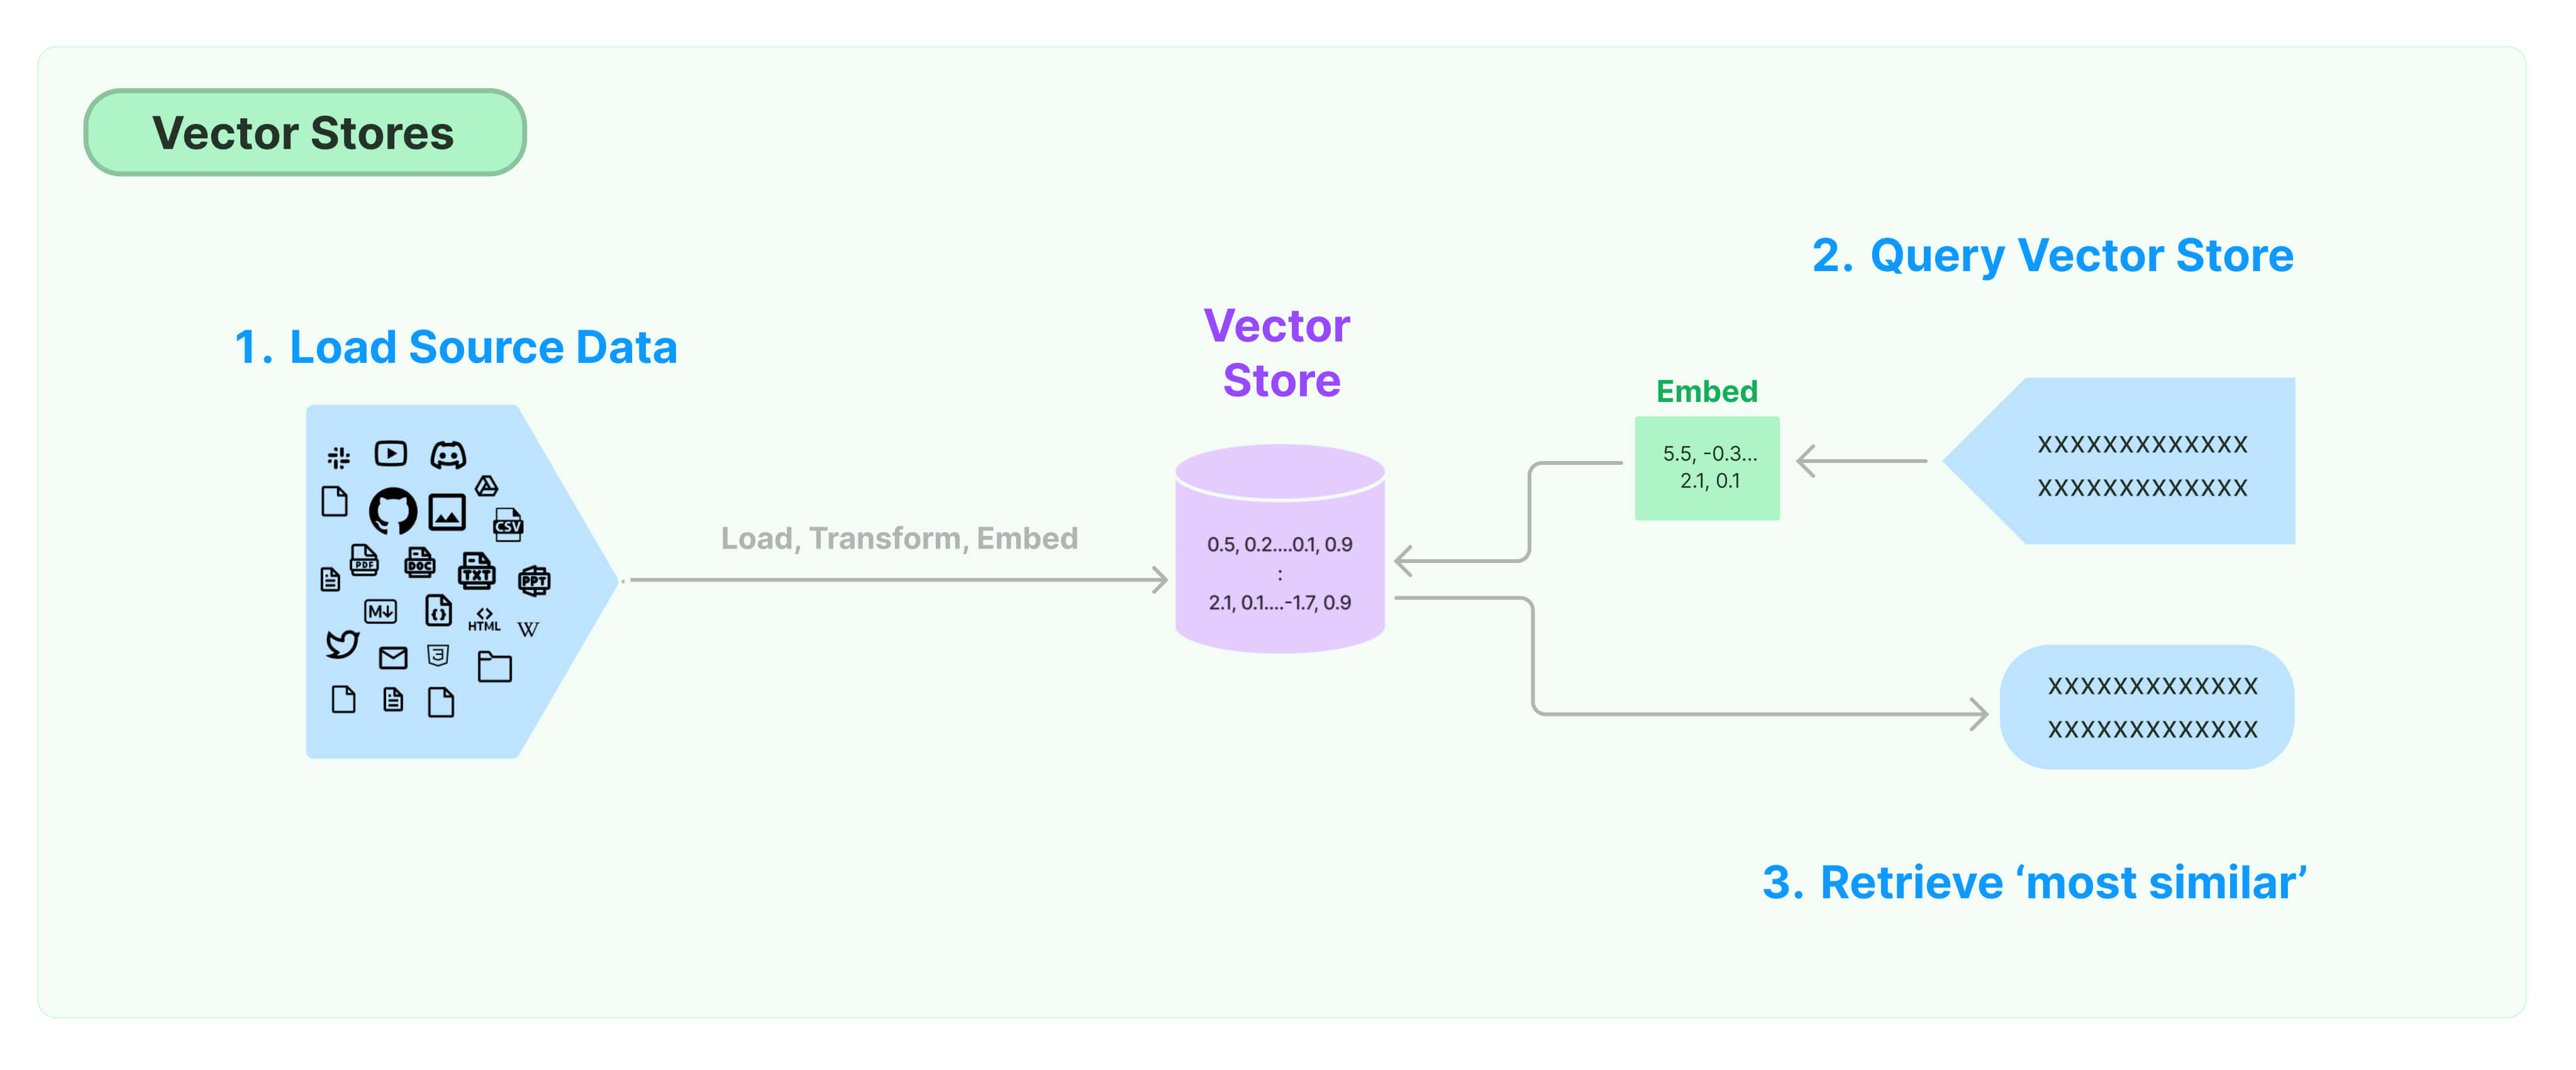
\includegraphics[width=\linewidth]{./figures/vectorstore.jpg}
    \caption{Vector Store Process Diagram \cite{langchainvectorstore}}
    \begin{flushleft}
        \small This figure illustrates the functioning of an embedding model in a vector store environment, transforming source data to numerical representations, and embedding queries to retrieve the most similar vectors.
    \end{flushleft}
\end{figure}
\subsection{Indexation}
The term indexation refers to the organization and storage of the generated embeddings to optimize the retrieval process afterwards. There are many indexation methods, such as Flat, Hierarchical, Quantized methods, etc... The exploration of these different methods is beyond the objectives of this internship, but these different indexation strategies share a common aim of storing chunks in a data structure, in a way that the similarity search algorithms (discussed below) can retrieve the relevant context efficiently and accurately.
\begin{figure}[H]
    \centering
    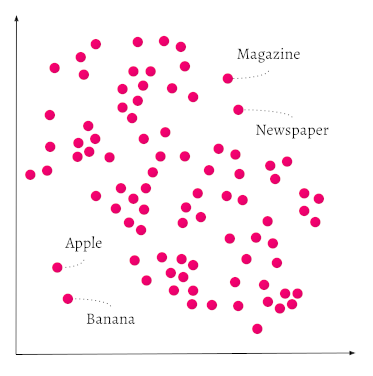
\includegraphics[width=.5\linewidth]{./figures/vs-indexation.png}
    \caption{Vector Store Index Visualization \cite{weaviateindexing}}
    \begin{flushleft}
        \small This figure demonstrates how some word embeddings are indexed so that semantically similar elements are grouped together.
    \end{flushleft}
\end{figure}
\subsection{Similarity Search}
In addition to the ability to index and store documents' sections in a suitable format, the vector store index should also be able to search these elements (and then decode them back into their original textual form). This is achieved through similarity search algorithms often implemented as constituent functionalities with the vector store. These functions return a number of passages semantically similar to the search term and is achieved due to the concept of distance calculation between vectors in data analysis.\newline
The following figure represents the different metrics of these algorithms.
\begin{figure}[H]
    \centering
    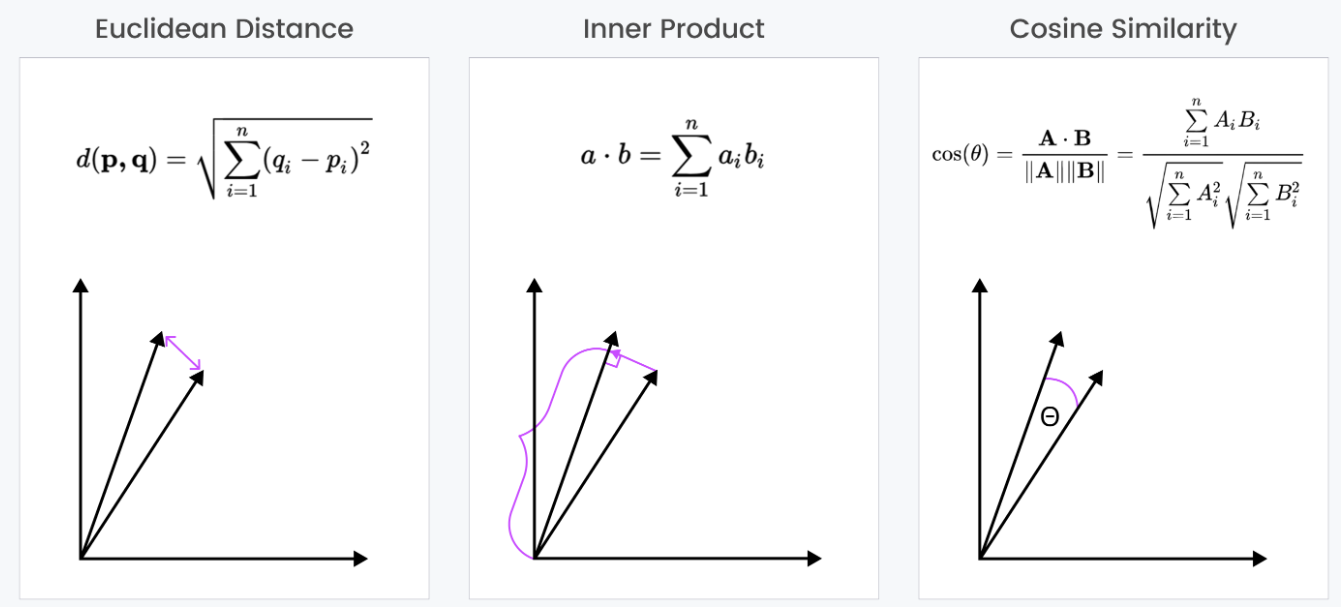
\includegraphics[width=\linewidth]{./figures/vector-distance-metrics.png}
    \caption{Similarity Metrics for Vector Search \cite{zsimilaritymetrics}}
\end{figure}
The Euclidean Distance metric is more suitable when looking for precise differences in numerical values, achieving results similar to exact word matching, which is irrelevant in the context of RAG. The Inner Product metric is more advanced in a way that it focuses on calculating the difference between the vectors' directions more than their magnitudes, but still it prioritizes results with similar lengths to the input query. The cosine similarity metric, which is the most suitable algorithm for our case, only calculates similarity based on the direction of vectors rather than their magnitude, which means that the embeddings which will be retrieved from the knowledge base will be the ones with the most semantic similarity, rather than length similarity, to the user-provided query embeddings.
\subsection{Retrieval Re-ranking}
Considering the context window limitation mentioned in the chunking subsection, and the complex task of retrieving the most relevant context, it is worth employing an additional step to the similarity search metrics mentioned in the previous subsection. This is because cosine similarity, even though an efficient metric for retrieving the context, still has limitations when dealing with complex natural language content.
\begin{figure}[H]
    \centering
    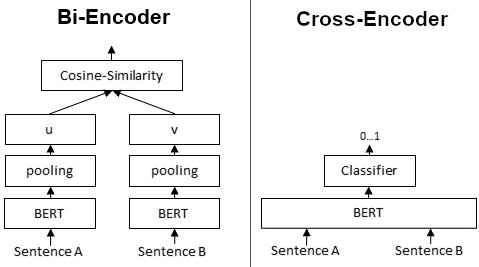
\includegraphics[width=.8\linewidth]{./figures/Bi_vs_Cross-Encoder.png}
    \caption{Bi-encoder VS Cross-encoder \cite{bivscrossencoders}}
\end{figure}
The post-retrieval process being discussed allows to compress the retrieved information from the basic similarity search algorithm by employing a neural network to further re-rank and drop irrelevant or recurrent parts from the retrieved information. This type of neural network, called Cross-Encoder Re-ranking, captures the order and relationships between the words in the query and the given chunk simultaneously, and predicts its relevance to the question.
\subsection{Large Language Models}
Text Generative AI encompasses models capable of artificially producing textual content based on a prompt (discussed in the following subsection). It can allude to the tasks of next word suggestions, summarization, rewriting in different tones, cross-language translation, question answering, text or code generation etc...
Large Language Models (LLMs) constitute a subset of AI models that leverage massive natural language training datasets. Prominent examples of such models include GPT-3, Gemini, and Llama-3. While some of these models have been extended to incorporate multimodal capabilities (multimedia content), their core functionality remains rooted in language processing and generation, providing a robust foundation for the required tasks in a RAG pipeline.
\begin{figure}[H]
    \centering
    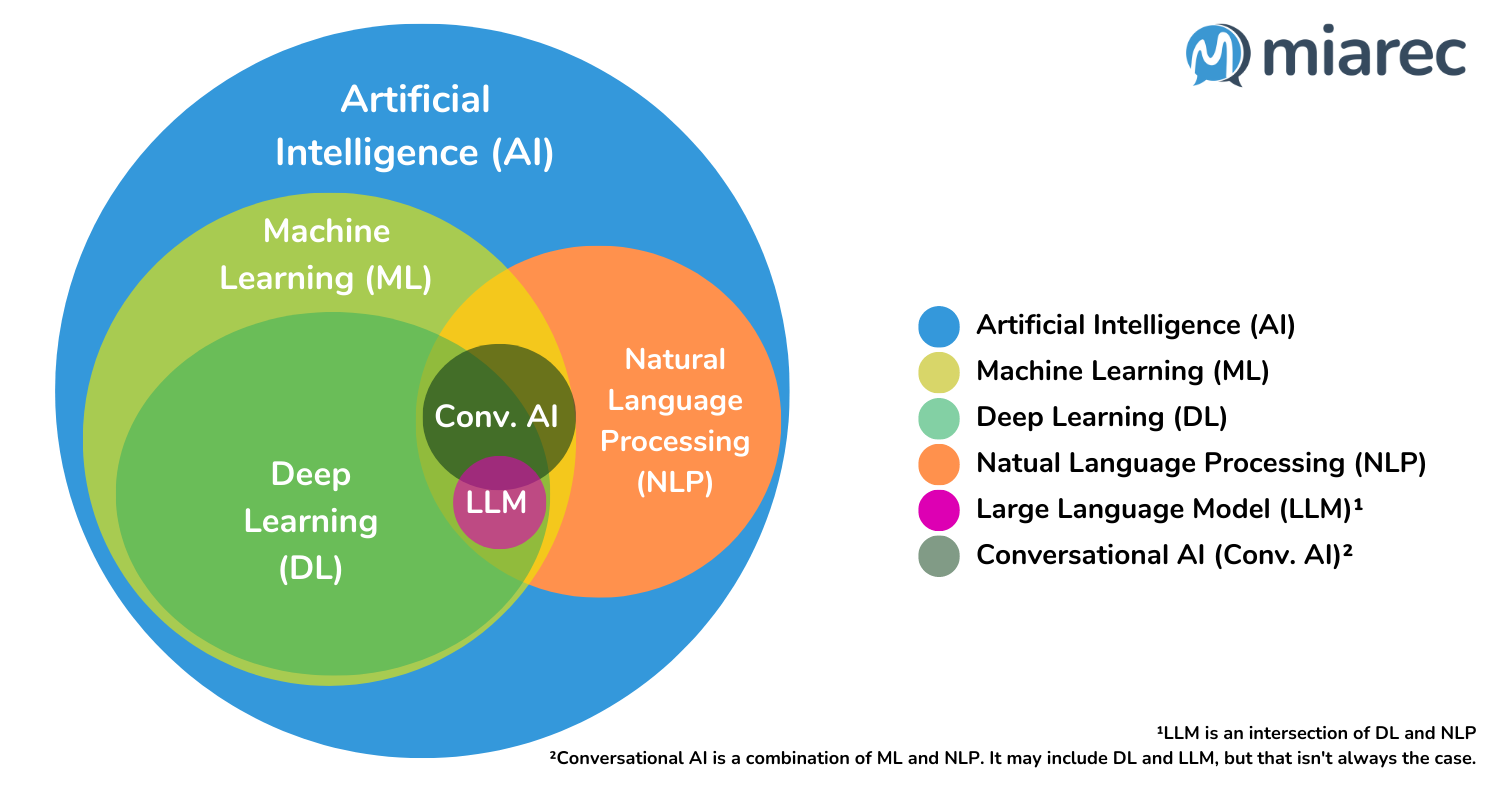
\includegraphics[width=.97\linewidth]{./figures/genai-relation-diagram.png}
    \caption{Relationship between AI, ML, DL, NLP, and Conversational AI terms \cite{aidomainsrel}}
    \begin{flushleft}
        \small This figure illustrates the relationship between AI domains. In this project, our focus is more onto LLMs (we use the term "LLM" interchangeably to mean "Large Language Model" that may or may not be "Conversational AI"), which are ML models able to hold chat history when answering consecutive queries.
    \end{flushleft}
\end{figure}
LLMs represent the principal component of a RAG system. It acts as tool that understands user prompts' context and generate textual responses accordingly. Essentially, these models are transformer-based, which allows them to learn complex relationships between words in sentences thanks to their attention mechanisms.
\begin{figure}[H]
    \centering
    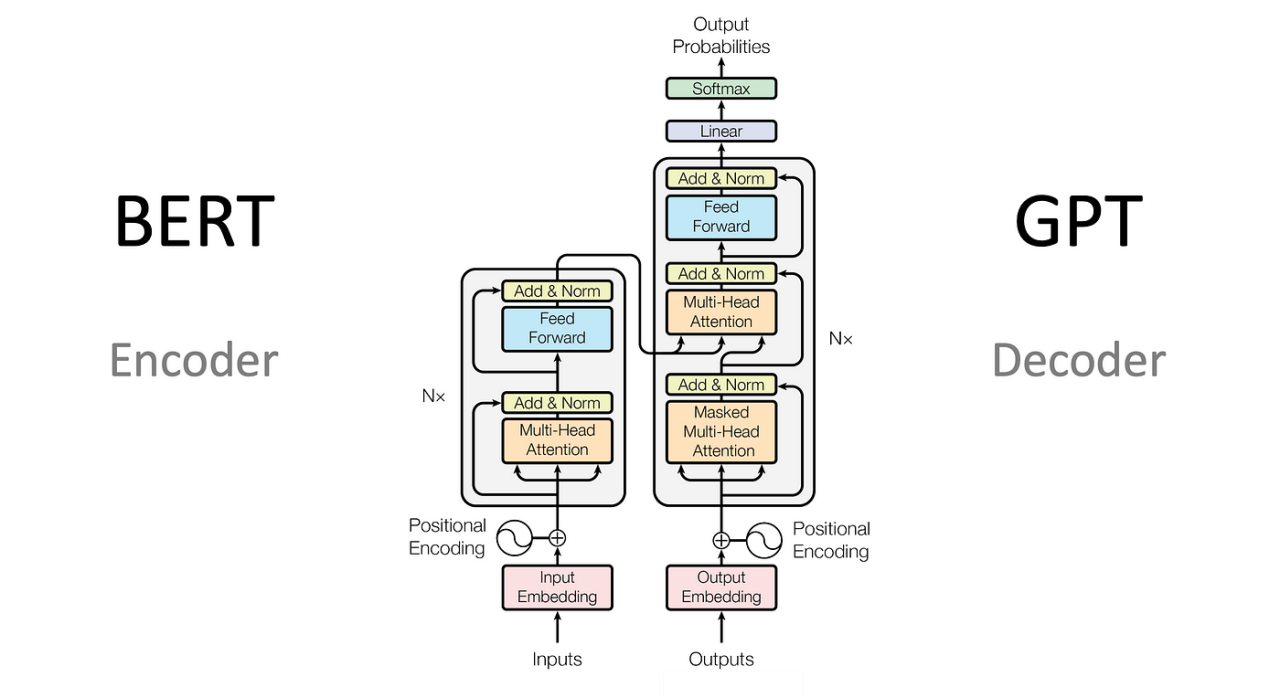
\includegraphics[width=\linewidth]{./figures/The-Transformer-model-architecture.png}
    \caption{An illustration of main components of the transformer model from the original paper \cite{transformersarch}}
\end{figure}
To provide some cursory understanding of the functioning of these models, the following are the main steps that such architecture involves:
\begin{itemize}
    \item \textbf{Input Embedding:} The transformer first converts the input text into a series of numerical representations,  which are then passed through a positional encoding layer. This layer adds information about the word’s position in the sentence, which is important because word order matters in a language like English.
    \item \textbf{Encoder Layers:} The core building block of the transformer encoder is the “encoder layer”.  An encoder layer typically consists of two sub-layers: a multi-head attention layer and a feed-forward layer.
    \item \textbf{Multi-Head Attention Layer:} The multi-head attention layer allows the model to attend to different parts of the input sentence simultaneously. This is important for understanding the relationships between words in a sentence.
    \item \textbf{Feed Forward Layer:} The feed-forward layer is a simple neural network that further processes the information from the attention layer.
    \item \textbf{Decoder Layers:} After the encoder has processed the input text, the decoder generates the output text. The decoder also uses encoder layers, but with an additional masked multi-head attention layer. This layer prevents the decoder from attending to future words in the output sentence, which would allow it to “cheat” by looking ahead.
    \item \textbf{Softmax Layer:} The softmax layer converts the decoder's output into a probability distribution over all the words in its vocabulary. This allows the model to predict the next word in the sentence for instance.
\end{itemize}
We can make use of these LLMs' capabilities and the retrieval phase discussed in the previous subsections, which when combined, serve to leverage the retrieved information to generate more insightful responses.
\subsection{Prompts and Prompt Engineering}
Prompt Engineering (PE) techniques play a crucial rule in the context of RAG and LLMs in general, by acting as a link between the retrieval and the generation phases. It refers to how the model is prompted, i.e. what does it receive as input. It may include several instructions to the LLM that guides it on how to perform the generation stage. It also can include different parts or steps, such as passing the retrieved context or chat history directly into the prompt, provide it with examples which it should consider when providing answers, or instruct it on how long the answer should be or in which tone it should respond.
\begin{figure}[H]
    \centering
    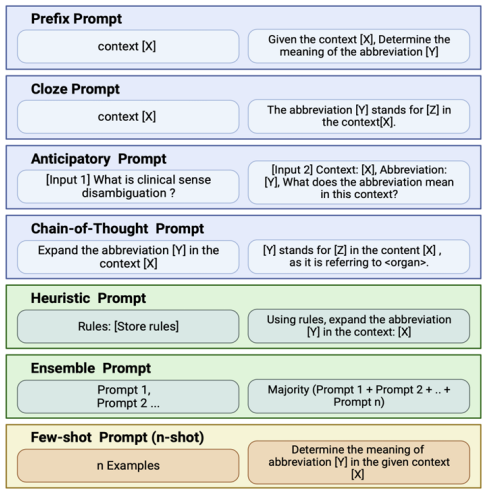
\includegraphics[width=\linewidth]{./figures/prompt-types.png}
    \caption{Types of Prompts: [X]: context, [Y]: Abbreviation, [Z]: Expanded Form
    \cite{prompts}}
    \begin{flushleft}
        The figure above provides many types and examples of prompts. We can distinguish two characteristics: instructions and placeholders.\newline
        Instructions, such as "Given the context [], Determine the meaning of []" and "Determine the meaning of [] in the given context []", allow to control how the AI model processes its input when generating answers, and help instruct the model to limit its knowledge based on the retrieved context for our case.\newline
        The placeholders, "[X]" and "[Y]" for example, allow to interpolate textual information that changes each time a model is called. These placeholders allow to insert user queries alongside our chosen instructions, and pass context relevant to the query each time, in format intelligible to the LLMs.
    \end{flushleft}
\end{figure}
\subsection{Generation Re-ranking}
This final post-generation phase process aims to prioritize better answers by calculating specific scores for each model's response generation. There are mainly three metrics for this type phase.
\subsubsection{Faithfulness}
This metric allows to measure the hallucination of a model and de-prioritizes its answer. It achieves this by calculating the proportion of the claims which can be inferred from the retrieved context against the total number of claims, which can be either from the context or not (hallucination).
\subsubsection{Answer Relevancy}
Similarly to the Faithfulness metric, which focuses on the generated answer its relation with the retrieved context, this metric assesses the pertinence of the generation phase's outcome to the initial prompt. This metric is calculated by reverse engineering the RAG pipeline: Given a generated answer, LLMs attempt to speculate some variants of questions that can be asked to obtain that generation, and then calculates the mean cosine similarity between those speculated questions and the actual question.
\subsubsection{Model Feedback}
This metric allows to capture the users' feedback and measure the trust our users have in AI models. It measures this by allowing each user to rate an answer in a scale from 1 to 5. These accumulated scores are then divided by the number of feedbacks given to a single LLM. In addition to this, a model which has no feedback is given a score of 3 to make it neither prioritized nor de-prioritized  over other models.

\section{Conclusion}
This chapter has identified the key components that will make up our system, highlighting the interaction between them. In summary, to implement a functional RAG pipeline, one needs to orchestrate a Vector Store with methods for knowledge augmentation, similarity search methods to retrieve relevant information, LLMs to generate responses, and prompt engineering to control LLMs' behavior.\newline
Having a clear understanding of these individual parts is essential, as the following chapter discusses the implementation phase in detail.